\section{Abordagens}
\begin{frame}{Aquisição do dataset}
  
  \begin{columns}

    \column{0.4\textwidth}
      \begin{figure}[h]
          \centering
          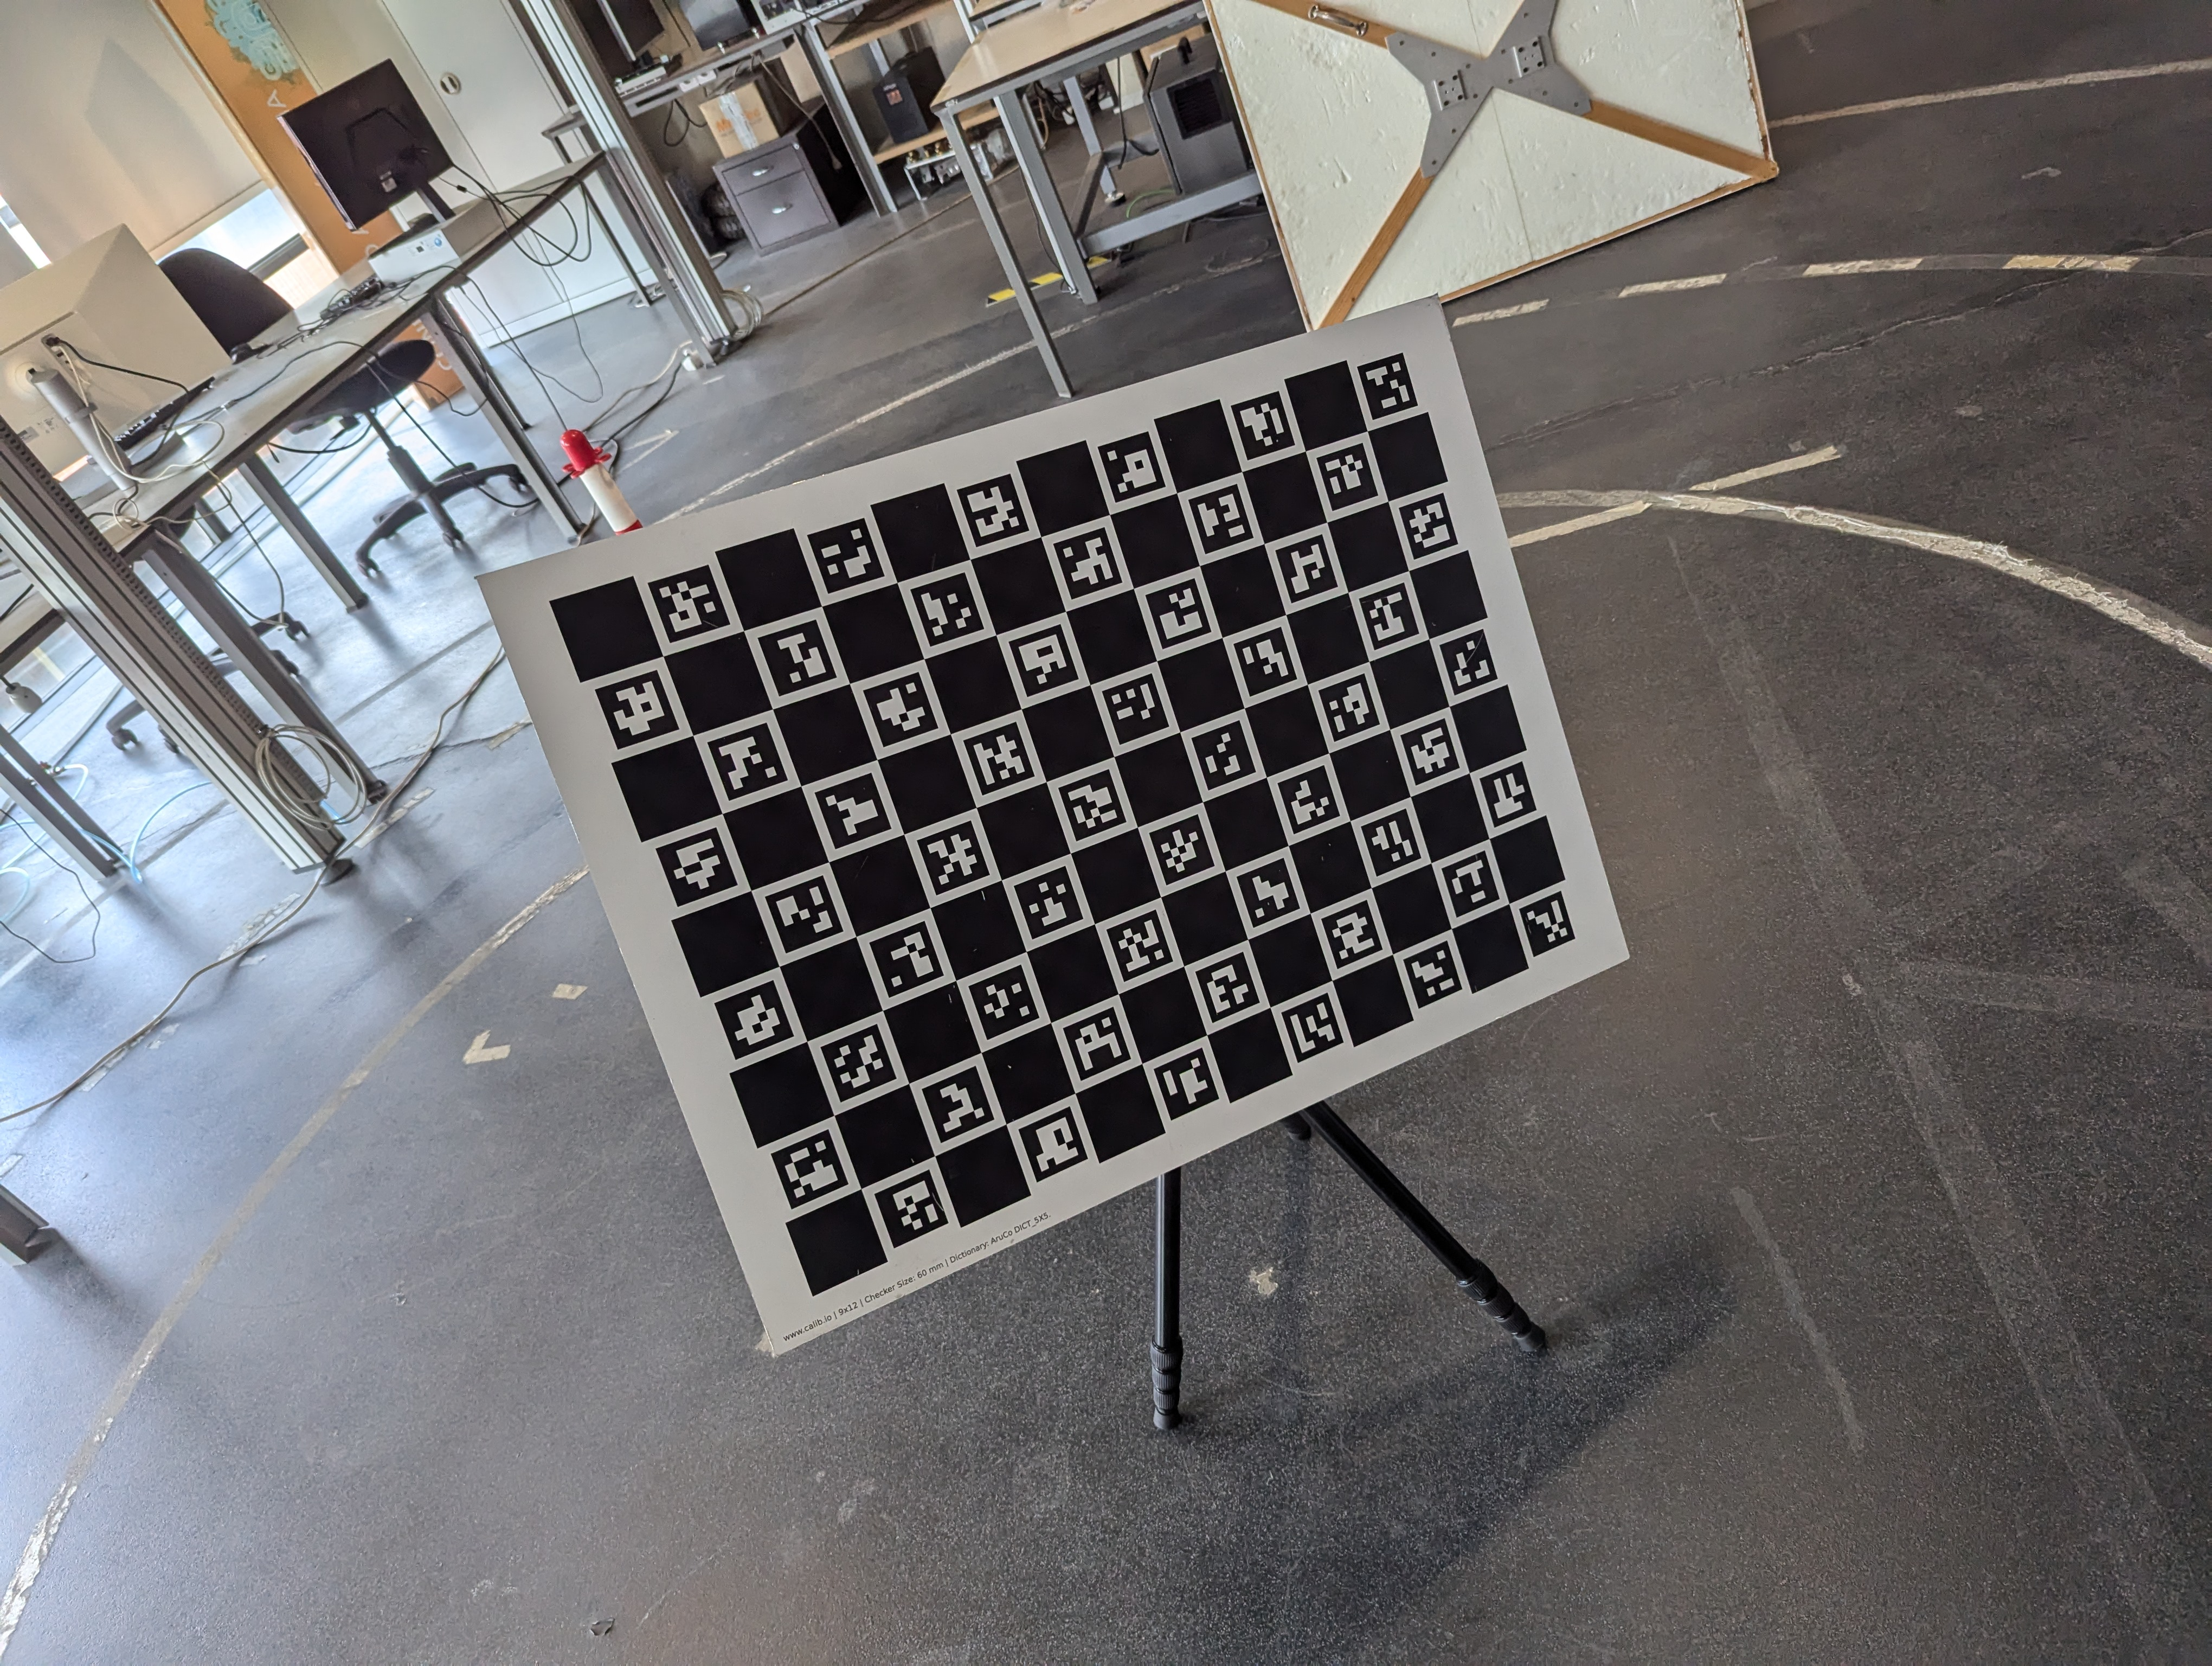
\includegraphics[width=0.9\textwidth]{resources/images/pattern_28.jpg}
          \captionsetup{labelformat=empty}
          \caption{Imagem original}
      \end{figure}
      % {\Huge\setstretch{1.0} Semântica\par}

    \column{0.4\textwidth}
      \begin{figure}[h]
          \centering
          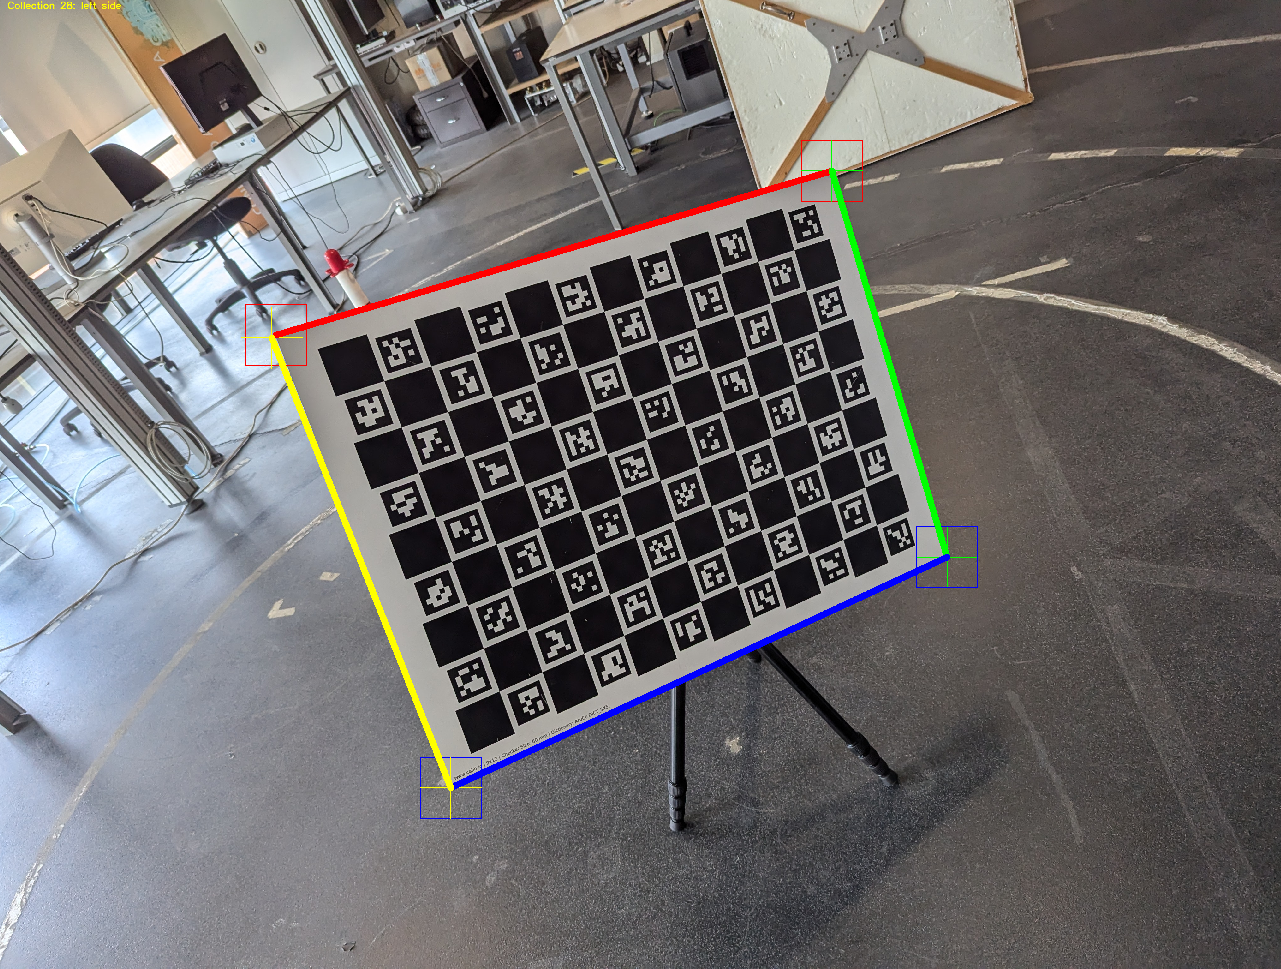
\includegraphics[width=0.9\textwidth]{resources/images/pattern_28_lines.png}
          \captionsetup{labelformat=empty}
          \caption{Anotações no ATOM}
      \end{figure}
  \end{columns}
      \vspace{\fill}
      \vspace{-0.2cm}


    % {\Huge\centering\setstretch{1.0} Panóptica\par}

      \begin{figure}[h]
          \centering
          
\includegraphics[width=0.36\textwidth]{resources/images/mask_pattern_28.jpg}
          \captionsetup{labelformat=empty}
          \caption{Conversão das linhas de contorno para uma máscara}
      \end{figure}
\end{frame}
\begin{frame}[c]{Seleção de modelos}{}

    \begin{itemize}
          \item Modelos pre-treinados do PyTorch
          \begin{itemize}
            \item DeepLabV3
            \item Fully Convolutional Network for Semantic Segmentation
            \item LRASPP
          \end{itemize}
          \item U-Net
    \end{itemize}

\end{frame}

\begin{frame}{Setup de treino}
  \begin{itemize}
    \item \textit{Loss function}: \textit{Binary cross-entropy loss}
    \item \textit{Optimizer}: Adam
    \item \textit{Batch size}: Máximo possível para a GPU
    \item Imagens com uma resolução de 512x512 pixeis
    \item 200 Épocas por treino
  \end{itemize}
  
\end{frame}